\section[Using git]{Example using git}
\begin{frame}
	\frametitle{Creating a git repository}
	\begin{columns}
		\begin{column}{0.4\textwidth}
			\begin{itemize}[<+->]
				\item New repository button
				\item Create the name
				\item Create a description
				\item Open or public?
				\item READMEs are cool
				\item Gitignore is useful
				\item Add license
			\end{itemize}
		\end{column}
		\begin{column}{0.6\textwidth}
			\begin{figure}
				\centering
				\begin{overprint}
					\onslide<1>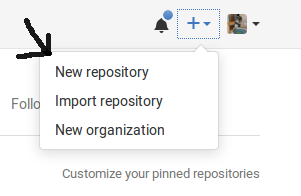
\includegraphics[width=\textwidth]{./pictures/new_repository.png}
					\onslide<2>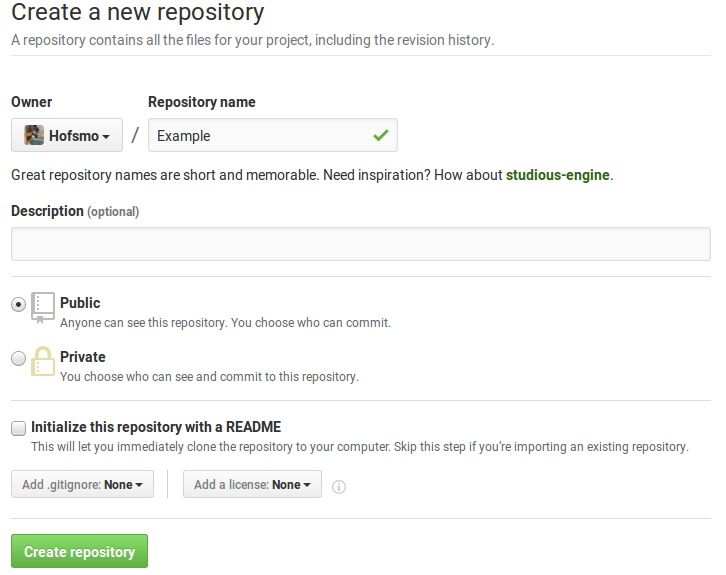
\includegraphics[width=\textwidth]{./pictures/rep_name.png}
					\onslide<3,4>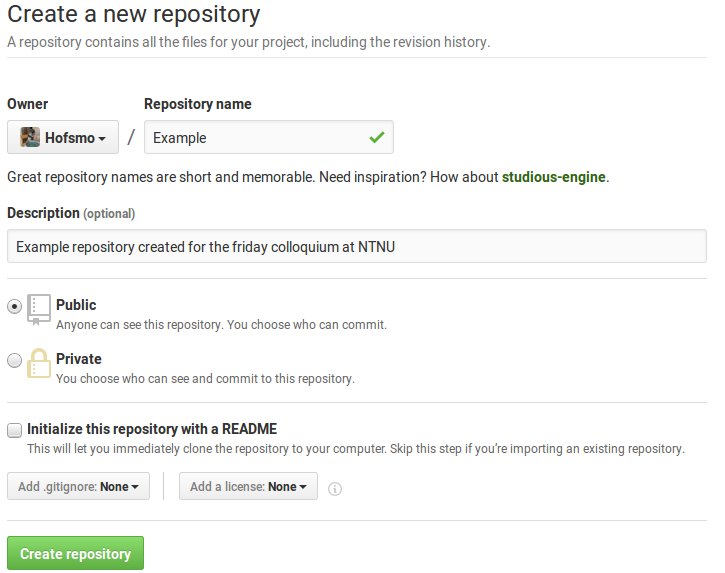
\includegraphics[width=\textwidth]{./pictures/rep_descr.png}
					\onslide<5>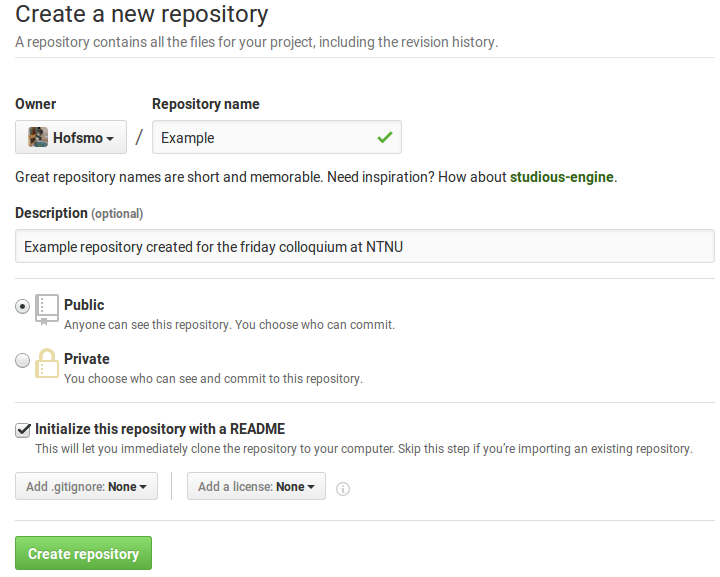
\includegraphics[width=\textwidth]{./pictures/rep_readme.png}
					\onslide<6>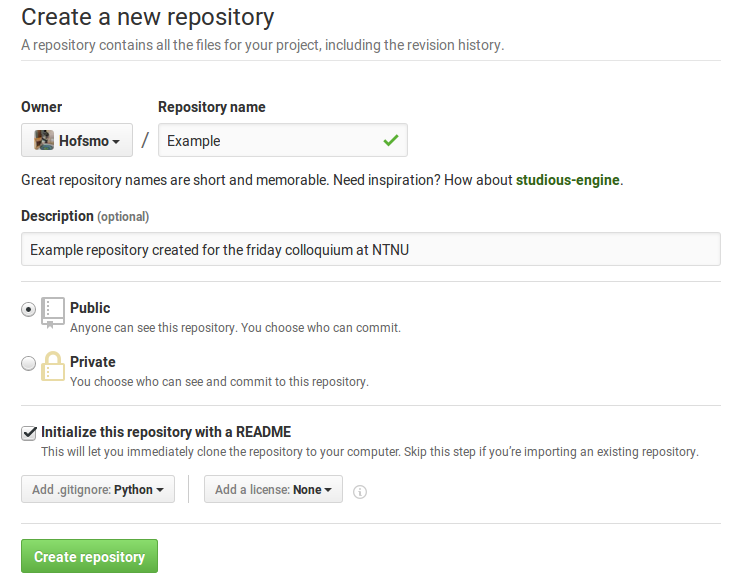
\includegraphics[width=\textwidth]{./pictures/rep_ignore.png}
					\onslide<7>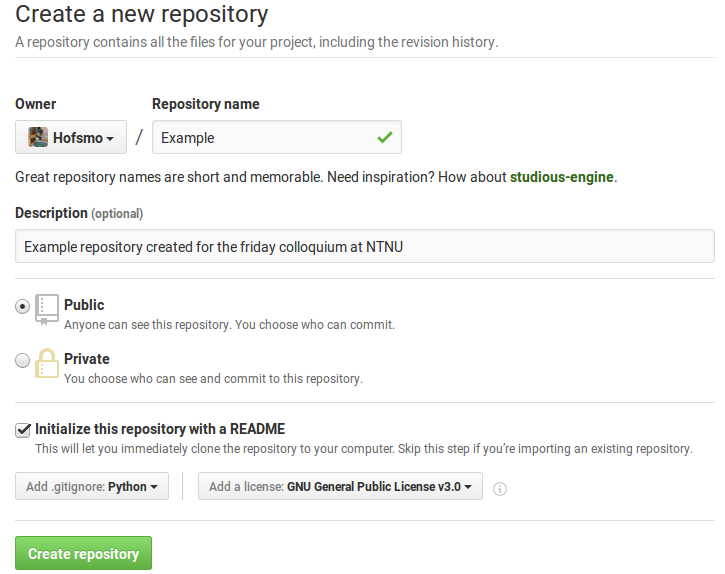
\includegraphics[width=\textwidth]{./pictures/rep_license.png}
				\end{overprint}
			\end{figure}
		\end{column}
	\end{columns}
\end{frame}
\begin{frame}
	\frametitle{Resulting repository}
	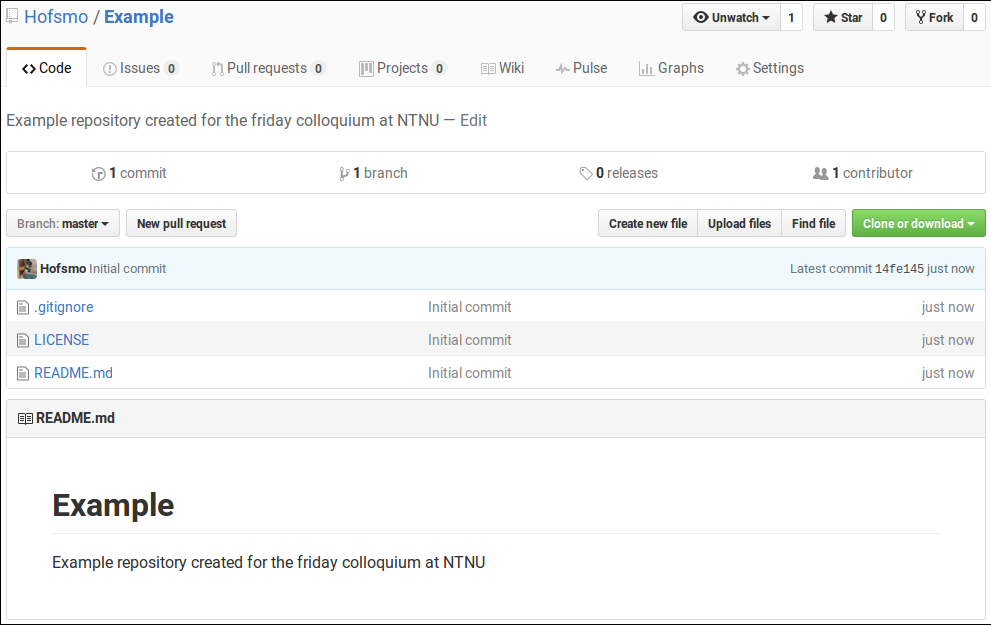
\includegraphics[width=\textwidth]{./pictures/repository.png}
\end{frame}
\begin{frame}
	\frametitle{Cloing the repository}
	\begin{columns}
		\begin{column}{0.4\textwidth}
			\begin{itemize}[<+->]
				\item using the terminal
					\begin{itemize}[<+->]
						\item Copy the url
						\item Run command
						\item Done
					\end{itemize}
				\item Using a GUI(GitKraken in this case)
					\begin{itemize}[<+->]
						\item Find clone repo button
						\item Select repository
						\item Decide where to put it and clone
					\end{itemize}
			\end{itemize}
		\end{column}
		\begin{column}{0.6\textwidth}
			\begin{figure}
				\centering
				\begin{overprint}
					\onslide<1>
\includegraphics[width=\textwidth]{./pictures/term.png}
					\onslide<2>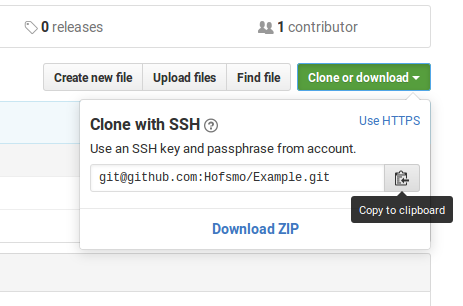
\includegraphics[width=\textwidth]{./pictures/copy_url.png}
					\onslide<3>
\includegraphics[width=\textwidth]{./pictures/clone_term.png}
					\onslide<4>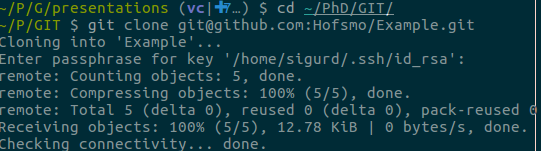
\includegraphics[width=\textwidth]{./pictures/term_cloned.png}
					\onslide<5,6>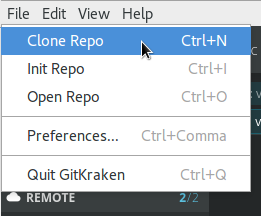
\includegraphics[width=\textwidth]{./pictures/kraken_file.png}
					\onslide<7>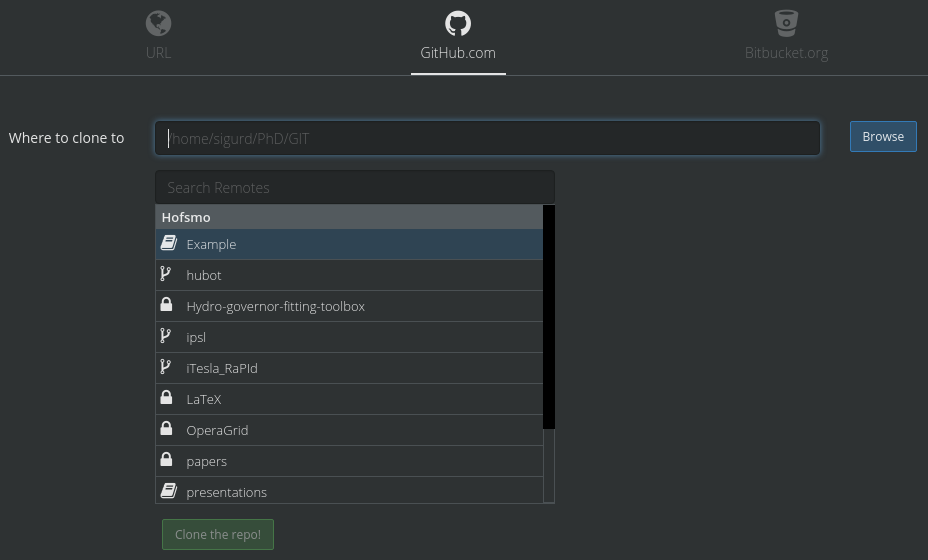
\includegraphics[width=\textwidth]{./pictures/kraken_example.png}
					\onslide<8>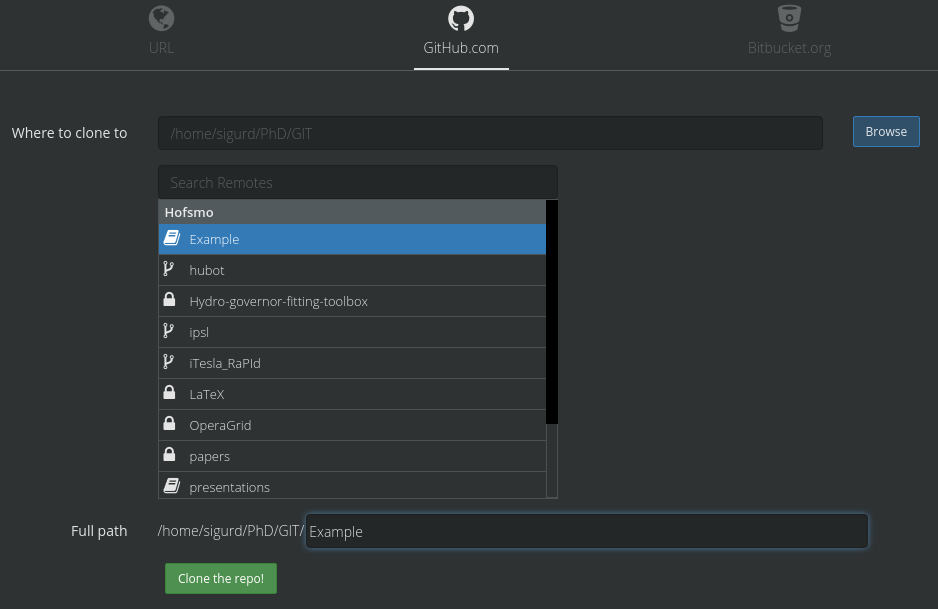
\includegraphics[width=\textwidth]{./pictures/kraken_clone.png}
				\end{overprint}
			\end{figure}
		\end{column}
	\end{columns}
\end{frame}
\begin{frame}
	\frametitle{Staging our first file}
	\begin{columns}
		\begin{column}{0.35\textwidth}
			\begin{itemize}[<+->]
				\item In the terminal
					\begin{itemize}[<+->]
						\item git status
						\item stage file using git add
					\end{itemize}
				\item In the GUI
					\begin{itemize}[<+->]
						\item Push "Stage File" button
					\end{itemize}
			\end{itemize}
		\end{column}
		\begin{column}{0.65\textwidth}
			\begin{figure}
				\centering
				\begin{overprint}
					\onslide<1,2>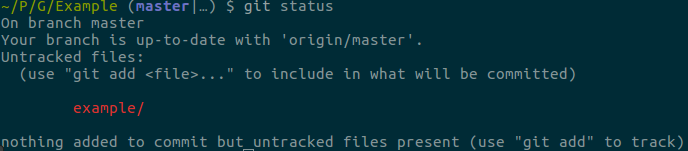
\includegraphics[width=\textwidth]{pictures/term_status.png}
					\onslide<3>
\includegraphics[width=\textwidth]{pictures/term_add.png}
					\onslide<4>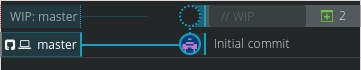
\includegraphics[width=\textwidth]{pictures/kraken_status.png}
					\onslide<5>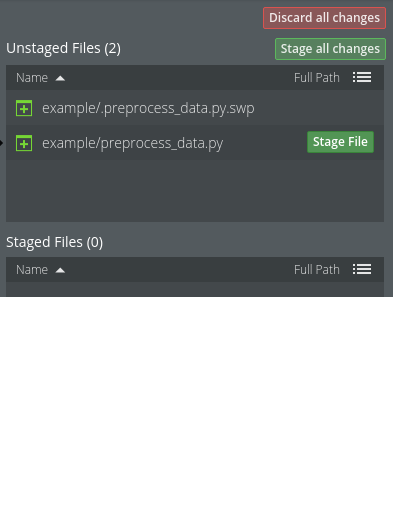
\includegraphics[width=\textwidth]{pictures/kraken_stage.png}
				\end{overprint}
			\end{figure}
		\end{column}
	\end{columns}
\end{frame}
\begin{frame}
	\frametitle{Ignoring editor generated file}
	\begin{columns}
		\begin{column}{0.4\textwidth}
			\begin{itemize}[<+->]
				\item Remember the second file?
				\item Tell git to ignore it
				\item Git ignores it
				\item Stage the modified .gitignore
			\end{itemize}
		\end{column}
	\begin{column}{0.6\textwidth}
		\begin{figure}
			\centering
			\begin{overprint}
				\onslide<1>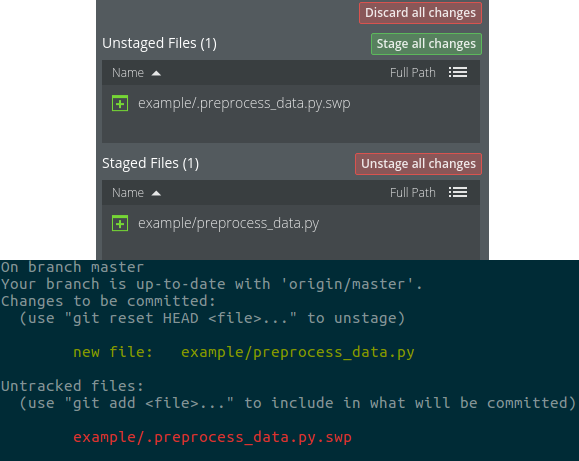
\includegraphics[width=\textwidth]{./pictures/to_ignore.png}
				\onslide<2>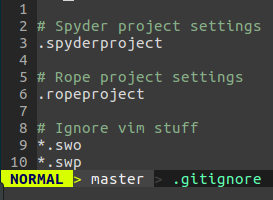
\includegraphics[width=\textwidth]{./pictures/gitignore.png}
				\onslide<3>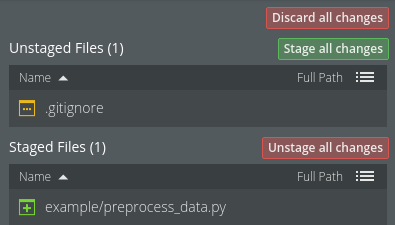
\includegraphics[width=\textwidth]{./pictures/ignored.png}
				\onslide<4>
\includegraphics[width=\textwidth]{./pictures/add_gitignore.png}
			\end{overprint}
		\end{figure}
	\end{column}
	\end{columns}
\end{frame}
\begin{frame}
	\frametitle{Our first commit}
	\begin{columns}
		\begin{column}{0.4\textwidth}
			\begin{itemize}[<+->]
				\item In terminal:
				\begin{itemize}[<+->]
					\item Enter git commit
					\item Write and save commit message
				\end{itemize}
				\item In GUI:
				\begin{itemize}
					\item Write commit message
					\item Push commit button
				\end{itemize}
			\end{itemize}
		\end{column}
		\begin{column}{0.6\textwidth}
			\begin{figure}
				\centering
				\begin{overprint}
					\onslide<1>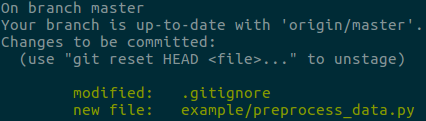
\includegraphics[width=\textwidth]{./pictures/status_before_commit.png}
					\onslide<2>
\includegraphics[width=\textwidth]{./pictures/git_commit.png}
					\onslide<3>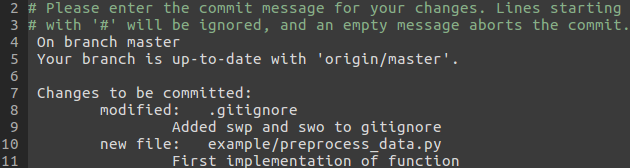
\includegraphics[width=\textwidth]{./pictures/commit_message.png}
					\onslide<4>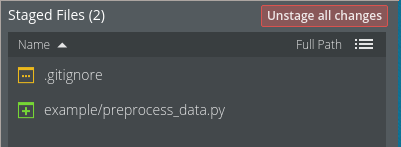
\includegraphics[width=\textwidth]{./pictures/kraken_before_commit.png}
					\onslide<5,6>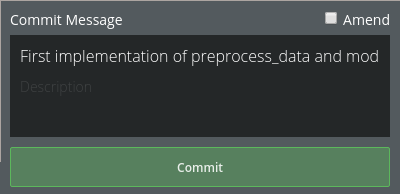
\includegraphics[width=\textwidth]{./pictures/kraken_commit.png}
				\end{overprint}
			\end{figure}
		\end{column}
	\end{columns}
\end{frame}
\begin{frame}
	\frametitle{Push the changes to GitHub}
	\begin{columns}
		\begin{column}{0.4\textwidth}
			\begin{itemize}[<+->]
				\item GitHub (remote) is now behind our local copy
				\item Push changes to GitHub
				\item GitHub and local copy are now equal
			\end{itemize}
		\end{column}
		\begin{column}{0.6\textwidth}
			\begin{figure}
				\centering
				\begin{overprint}
					\onslide<1>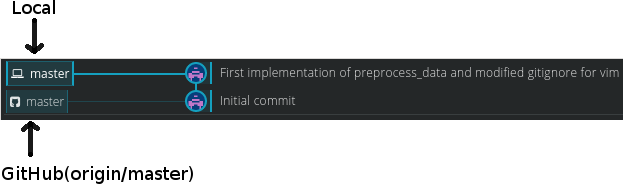
\includegraphics[width=\textwidth]{./pictures/first_commit.png}
					\onslide<2>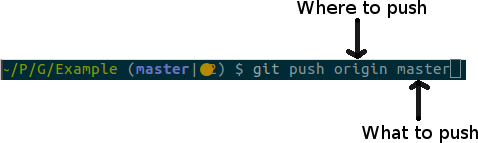
\includegraphics[width=\textwidth]{./pictures/git_push_master.png}
					\onslide<3>
\includegraphics[width=\textwidth]{./pictures/synced.png}
				\end{overprint}
			\end{figure}
		\end{column}
	\end{columns}
\end{frame}

		
